% REMEMBER: You must not plagiarise anything in your report. Be extremely careful.

\documentclass{l4proj}

    
%
% put any additional packages here
%

\begin{document}

%==============================================================================
%% METADATA
\title{Level 4 Project Report}
\author{Gemma McDonald}
\date{January 28, 2021}

\maketitle

%==============================================================================
%% ABSTRACT
\begin{abstract}
    Every abstract follows a similar pattern. Motivate; set aims; describe work; explain results.
    \vskip 0.5em
    ``XYZ is bad. This project investigated ABC to determine if it was better. 
    ABC used XXX and YYY to implement ZZZ. This is particularly interesting as XXX and YYY have
    never been used together. It was found that  
    ABC was 20\% better than XYZ, though it caused rabies in half of subjects.''
    \vskip 0.5em
    Explain a little bit about the background of the subject\newline
    What is it i have worked on and what i have done for it
    Graduate attributes and what they are
    What i made and what effect i think this will have
    Evaluated
    What was found
    Why this is useful
    What can be done to further improve this research
\end{abstract}

%==============================================================================

% EDUCATION REUSE CONSENT FORM
% If you consent to your project being shown to future students for educational purposes
% then insert your name and the date below to  sign the education use form that appears in the front of the document. 
% You must explicitly give consent if you wish to do so.
% If you sign, your project may be included in the Hall of Fame if it scores particularly highly.
%
% Please note that you are under no obligation to sign 
% this declaration, but doing so would help future students.
%
\def\consentname {Gemma McDonald} % your full name
\def\consentdate {28 January 2021} % the date you agree
%
\educationalconsent


%==============================================================================
\tableofcontents

%==============================================================================
%% Notes on formatting
%==============================================================================
% The first page, abstract and table of contents are numbered using Roman numerals and are not
% included in the page count. 
%
% From now on pages are numbered
% using Arabic numerals. Therefore, immediately after the first call to \chapter we need the call
% \pagenumbering{arabic} and this should be called once only in the document. 
%
% Do not alter the bibliography style.
%
% The first Chapter should then be on page 1. You are allowed 40 pages for a 40 credit project and 30 pages for a 
% 20 credit report. This includes everything numbered in Arabic numerals (excluding front matter) up
% to but excluding the appendices and bibliography.
%
% You must not alter text size (it is currently 10pt) or alter margins or spacing.
%
%
%==================================================================================================================================
%
% IMPORTANT
% The chapter headings here are **suggestions**. You don't have to follow this model if
% it doesn't fit your project. Every project should have an introduction and conclusion,
% however. 
%
%==================================================================================================================================
\chapter{Introduction}

% reset page numbering. Don't remove this!
\pagenumbering{arabic} 

Graduate attributes, also referred to as 'soft' skills, encompasses all the abilities 
developed by students during their time in university that are not directly related to
their chosen degree. These skills increase a students’ employability, allows them to 
integrate better into the workplace and creates a better environment within teams. However,
due to a lack of understanding of these skills, they are often overlooked by universities.
\par 
We believe there is the potential for encouraging the development of these skills through
the use of a mobile application. This project explores how the use of this app, with the
integration of Cognitive Behavioural Therapy (CBT) techniques, could increase awareness 
of when these skills are being used, and developing them through reflection. We will 
present the existing relevant research, and outline the process of creating this 
mobile application including the requirements, the design of the app, and how it was 
implemented.
\par 
We will then present an evaluation using a prototype app created for iOS. The results of
this evaluation and how they relate to the literature we be discussed, as well as the 
conclusions that can be drawn relating to the impact this app could have on the development
of 'soft' skills within students.
\par 
This chapter will introduce the GradReflect project, outlining the motivations and aims 
for creating an app to aid reflection on graduate
skills, and will present the research aims that this project will address.

\section{Motivation}
The importance of graduate attributes (also referred to as ‘soft skills’) is not a 
novel idea within the literature. (Reference) found that industries are less concerned
about the technical skills that graduates enter the job with than the soft skills they have.
The importance of these skills is repeatedly expressed within research, illustrating that 
despite the expectation on tertiary education to provide students 
with these skills, graduates are being found to be underprepared to join the workplace 
(reference). 
\par 
This is potentially due to the requirement of reflection on real-life experiences 
being necessary for major development (reference), making these skills difficult to teach
through conventional teaching methodologies. Additionally, universities have been found to
believe that the demand for the teaching of these skills by industry professionals is 
purely a desire for universities to teach what is curently 'fashionable'. However, this
is not the case as these skills have been shown to allow graduates to integrate better 
into the workplace and create a better working environment within teams (reference).
This gap in understanding of how to teach these skills and the misconceptions surrounding
them has made universities and their academics resistant to integrate these skills into 
the teaching model. 
\par 
However, new methodologies have been presented 
to assist in the development of these skills within students, such as real-world 
projects and reflection diaries.
\par 
The potential to create an application that encourages users to reflect on their 
real-world experiences could increase awareness of these skills within students, 
encouraging their development and increasing their likelihood of success within the 
workplace, which is often a source of concern for students (reference).

\section{Aims - further work needed on the aims}
In light of the above motivations, we will build an iOS mobile application that will enable
students to capture their reflections on situations where they have exercised their 
graduate skills, encouraging the awareness and development of these skills. This 
application will incorporate CBT techniques to prompt deeper and more meaningful 
reflections. 
\par 
An initial exploratory study will be carried out to determine whether using Cognitive 
Behavioural Therapy (CBT) techniques are a viable method to encourage reflections within 
students. The results of this experiment will be analysed to answer the question: 
Does CBT benefit reflection by students on their graduate skills?
\par 
An evaluation will then be conducted using the application to address the need for 
students to have a space they can capture their reflections in a convient and simple way
that they will be likely to continue using. 
\par 
This evaluation will hope to give insight into whether the following goals have been met:
\begin{itemize}
    \item \textbf{Create an application to capture reflection on graduate attributes:} The
    main goal of this project is to create an application that provides allows 
    users to make reflections on how they have developed their graduate attributes.
    \item \textbf{Allow users to create a note via written or audio form:} The app must 
    allow users be able to quickly make a note of how and when they have used these 
    skills in a method that is most quick and convenient for them.
    \item \textbf{Capability for reminders:} Reflecting is a vital part of developing these
    skills, however, finding the time to do this is difficult. The application therefore
    must allow reminders so users know when they need to reflect.
    \item \textbf{Create a usable application:} Creating a usable application will 
    encourage repeated use by users, if users find the application attractive and satisfying
    to use then it increases the usability.
    \item \textbf{Aid reflection} The evaluation will also hope to answer whether the 
    application aids reflection for the users and encourages deeper reflections. This 
    project hopes to encourage users to continue using the application to reflect.
\end{itemize}


\section{Summary}
The remainder of the paper will discuss how the motivations for GradReflect was developed
into a working system, and how the aims were met.
The paper is structured as follows:
\begin{itemize}
    \item
    \textbf{Chapter 2} discusses
    \item
    \textbf{Chapter 3} discusses
    \item
    \textbf{Chapter 4} discusses
    \item
    \textbf{Chapter 5} discusses
    \item
    \textbf{Chapter 6} discusses
    \item
    \textbf{Chapter 7} discusses
    \item
    \textbf{Chapter 8} discusses
    How this project could be used in the future - that people could use the app for an extended period of 
time to really test out if it improves skills
That student could be encouraged by universities to use an app such as this by their universities
\end{itemize}



\section{Guidance}

\section{Writing guidance}
\begin{itemize}
\item If you are referring to a reference as a noun, then cite it as: ``\citet{Orw68} discusses the role of language in political thought.''
\item If you are referring implicitly to references, use: ``There are many good books on writing \citep{Orw68, Wil09, Pin15}.''
\end{itemize}


%==================================================================================================================================
\chapter{Background}


\section{General plan}

Description of the background chapter
what did other people do, and how is it relevant to what you want to do?
Don't give a laundry list of references or other software. Tie everything you say to your problem.
THink critically, weigh up how the background is contributing the my research and my project.
This is the major lit review, so start with that one and build massively - the RMT lit review will need a lot of detail about CBT added to it
Go into detail about everything that is relevant to the project
\par 
Maybe start by discussing graduate attributes and start with matthew barr paper. 
THen discuss the benefits these skills have again but relate it to the research papers that have been 
read, give examples of using these skills. Quote from people saying it is valuable.
HERE IS WHERE THE RMT LIT REVIEW MAY COME IN
\par 
Then discuss in detail how these skills are developed and the research that supports this .
Discuss other ways people have previously tried to introduce these skills and devlop them 
\par 
Start to go into detail about reflection itself and the research into it.
Discuss the research that went into having students reflect and how it improved their skills. Discuss about
how reflection generally just helps you learn and assimilate your skills. 
Discuss the different levels of reflection that have been created.
Discuss about how people need to be doing this reflection over a period of time to get the full benefits.
\par 
Start introducing CBT as a concept
THen discuss how CBT benefits its users and what it involves
What are the stages of CBT and how do people do it, start introducing the tools that people use.
Then can mention how closely it links to the stages of relfection that users should carry out to 
assimilate and develop their graduate attributes. 
TRY TO SEE IF THIS HAS BEEN DONE BEFORE AND IF NOT CAN MENTION THAT IT HAS NOT BEEN DONE BEFORE. 
\par 
Other apps that are similar. So here start to discuss other applications that encourage reflection 
what i learned fromt them.
Include pics of the main page of all of them.
Discuss the glasgow uni moodle one, the quarentine family video interview site that i researched,
Reflectly app that uses Artificial Intelligence. How does it help? Them maybe start to discuss the pros and 
cons of each one, did i take any inspiration from them. 
\par 
What are the best methods of interaction? Text or speech? Discuss the benefits to both, text is similar 
to CBT, but then speech can be useful to as talking can sometimes make it easier to get words across. In
CBT the participant would actually be using both techniques, they would have their journal but they 
would also have their sessions with the therapist. Include that nature by having both. Ability to use speech If
they cant in that moment to text but they have the option to convert it or just keep it. This will in itself
develop the communication skills as over time by using recordings they are having to develop their method
of getting across their ideas and getting more comfortable doing this. So with time the app could increase their
skills in ways other than just reflection. Also creates confidence in their ability to discuss their 
skills which will help them in future job interviews and potentially in the workplace as they will be more 
comfortable voicing out loud their skills and could give them the confidence to be able to take on new tasks.
Maybe discuss for a tiny bit about imposter sydrome being very prominent. Having a place where someone has to 
reflect on what they are good at or be honest about what needs to be developed could be very important and
help them overcome this. 
\par 
Potentially then start to discuss the benefits of seeing the statistics? Get insight into what you are 
developing
\par 
Maybe a section on potential issues that may come up during the creation/use of the app that i will want to 
overcome - novelty? 



\section{LIT REVIEW from RMT} 

The importance of graduate attributes (also referred to as ‘soft skills’) is not a novel idea 
within the literature. This importance is repeatedly expressed within research which illustrates 
that, despite the expectation on tertiary education to provide students with these skills, graduates 
are being found to be underprepared to join the workplace. These skills have been found to be 
difficult to teach through conventional teaching models, due to the need of real-life experiences 
being required for major development of them, making universities and their academics resistant to 
integrating the teaching of these skills into the teaching model. However, new methodologies have 
been presented to assist in the development of these skills within students, such as real-world 
projects and reflection. \textbf{Come back to reference}
\par  
Barr [1] provides a good introduction into the concept of graduate attributes and 
how these skills are developed within tertiary education. Barr lists these skills as involving 
problem-solving, critical thinking and self-organisation and states their importance to increasing 
a students’ employability. He discusses that while these skills are expected to be learned during a 
students’ time at university, these skills are not necessarily a causality of the courses the student 
undertakes. These attributes are often neglected as they are viewed as tacit due to the gap in 
understanding of what these skills are or how they could be taught. Barr suggests that this is a 
failing of tertiary education and seeks to provide a method to learn these skills and further develop them through the use of video games. 
The necessity of these soft skills which are required for employability are also discussed in 
the works of Stevens and Norman [4], echoing Barr. Through research involving surveying job 
advertisements and interviewing industry representatives, these authors helped to create a deeper 
understanding of why these attributes are desired by employers. Their work was able to refute 
claims made by universities that industry was looking for academics to teach what was fashionable, 
and instead showed that by having these skills graduates were able to integrate better into the 
workplace, increase their productivity and create a better environment within teams.  Of the 20 
industry representatives interviewed, every interviewee was insistent that soft skills are 
beneficial in the workplace but graduates often are underdeveloped and not work-ready. Students 
were also found to find that when graduates they felt their technical skills were not enough to 
secure them employment. This paper shows how vital these skills are within the real-world and the 
detrimental effect it can have on students if universities do not adequately develop these skills 
during their education.
\par 
Despite the importance of universities to teach these skills, there is little support to 
help academics understand what these skills are and how they could be integrated into the curriculum.
 Litchfield et al [2] attempt to resolve this problem through the creation of a project website 
 containing advice and activities for education on graduate attributes. However, this site was not 
 made permanent, meaning there is again a lack of resources to assist in the revision of the 
 teaching model within tertiary education.
 \par 
Abernathy and Treu [3] build upon the idea that real-world experiences are vital to the 
development of soft skills. The authors organise a course in cooperation with industry customers 
to give students the opportunity to be involved in a software development project from beginning 
to end. Over the duration of this course students had to develop both their communication and 
interpersonal skills to effectively handle both the client and their team. This real-world 
development of graduate skills was explored further through the works of McDermott et al [5] who 
used social blogs to aid in the development of soft skills within their students. The reflection 
that students were tasked with undertaking about their learning encouraged them to develop their 
critical thinking and self-sufficiency as they were required to monitor their own progress. 
However, this study found that students struggle to reflect and are not provided the necessary 
support needed to reflect effectively. 
\par 
Universities have been largely found to not provide adequate opportunity for students to 
develop the necessary graduate skills that will prepare them for the workplace. However, there is 
little support given for academics to integrate this within the teaching model. Methodologies such 
as video games, real-client development projects and social blogs have been found to develop some 
soft skills within student, but they do not provide a holistic approach to the development of 
these skills. It is necessary that these methodologies be combined in order to effectively 
develop these skills within students, and provide them with the tools to secure a happy and 
productive environment within the workplace.

%==================================================================================================================================
\chapter{Exploratory Study}
What is the problem that you want to solve, and how did you arrive at it?
Could potentially be a section to discuss the experiment that answers the research question 


%==================================================================================================================================
\chapter{Analysis/Requirements}
What is the problem that you want to solve, and how did you arrive at it?
\section{Guidance}
Make it clear how you derived the constrained form of your problem via a clear and logical process.
What is the problem that you want to solve, and how did you arrive at that?
Make it clear how you derived the constrained form of your problem via a clear and logical process. 
\par
So discuss who presented this problem, that we decided what was going to be included in this app 
iteratively throughout the weekly sessions, that i used lecture noes from MHCI and HCI
Further requirements gathered during a surevy that gained insight inot general understanding of grad attributes
and knowledge of their uses.
\par 
Discuss the user scenarios created and how they helped me decide what i needed to have in the app
User stories
\par 
The go onto the actual probelm statement and so use the question from the project options.
\par 
Do a section on functional requirements - use the moscow method
So use must have and Should have
\par 
Non functional requirements
General aspects rather than specific features that help to create and enjoyable experience
Also use the moscow method
\par 
Then discuss the limitations. things i would not be able to do.
So couldnt do moodle, what do i assume about the users. 
\par 
Discuss changes i made to the specification. This here is mainly about the moodle aspect but i can discuss 
that instead i opted for a link to sign into moodle if you want to go to a forumn to upload the reflections. 

%==================================================================================================================================
\chapter{Design}
How is this problem to be approached, without reference to specific implementation details? 
\section{Guidance}
Design should cover the abstract design in such a way that someone else might be able to do what you did, 
but with a different language or library or tool.
How is this problem to be approached, without reference to specific implementation details.
Design should cover the abstract design in such a way that someone else might be able to do what you did, 
but with a different language or library or tool.
\par 
Discuss the stuff from unit 3 and elsewhere of Mobile HCI - Interaction design, talk about the process of 
design, ie the design funnel, app definition statement, all the different design steps and diagrams
\par 
Do an overview, what is the app going to do.
\par 
Technical design - i used swift the language with swiftui interface lifecycle in an iOS mobile application.
For backend data storage i used Core data. THen talk a little bit about how this works too.
What language am i going to use, talk about why i chose swift. Talk about why swift has good interaction
as it is famous for having good interfaces, i am familiar with iOS interfaces as i use them myself.
Can do a page which shows the design of the views and how you naviagte between them in a diagram.
\par 
Do a section for each of the must haves and could haves that discuss exactly how i was going to go about 
designing and achieving that, they must directly correspond to the moscow requirements to provide proof.
Basically just going through every important aspect of the app and giving details on how i went about designing 
it. 
\par 
Can add wireframes here i think. Add in the drawing i had for the intial interface designs,
Talk about the user interface design process, mock up some wireframes of the initial looks that it had. Include
some of the pics from the old videos i have of the app interface as screenshots
How did i keep consistency throughtout the app, how did i keep it consistent with regular iOS practices.



%==================================================================================================================================
\chapter{Implementation} \label{implementation}
What did you do to implement this idea, and what technical achievements did you make?
You can't talk about everything. Cover the high level first, then cover important, relevant or impressive details.

What did you do to implement this idea, and what technical achievements did you make?
\section{Guidance}
You can't talk about everything. Cover the high level first, then cover important, relevant or impressive details.

\par 
Discuss the resources used. I used some online tutorials to get started and figure out how to use the design.
\par 
Then go on to discuss each component of the application and how it was created and what all the aspects do
together to create the full app. 
\par 
Do a section based on how the user interfaces were designed and created and what they involve and the view 
controlling and how they are all stored. Discuss views and the other types of code ie- the data models. How 
views are stored in the @State values. etc 
\par 
Do a section on the written note taking and how this works and interacts with core data.
\par 
Do a section on the voice recordings and how all of it works and where it saves etc.
\par 
Do a section on the statistics 
\par 
Do a small section on the aspects of the settings page and whats included in there.


\section{General points}

These points apply to the whole dissertation, not just this chapter.



\subsection{Figures}
\emph{Always} refer to figures included, like Figure \ref{fig:relu}, in the body of the text. Include full, explanatory captions and make sure the figures look good on the page.
You may include multiple figures in one float, as in Figure \ref{fig:synthetic}, using \texttt{subcaption}, which is enabled in the template.



% Figures are important. Use them well.
\begin{figure}
    \centering
    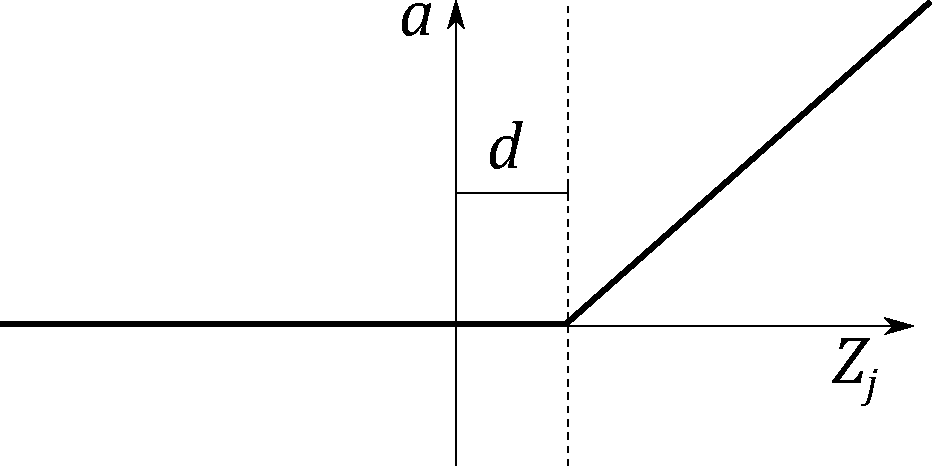
\includegraphics[width=0.5\linewidth]{images/relu.pdf}    

    \caption{In figure captions, explain what the reader is looking at: ``A schematic of the rectifying linear unit, where $a$ is the output amplitude,
    $d$ is a configurable dead-zone, and $Z_j$ is the input signal'', as well as why the reader is looking at this: 
    ``It is notable that there is no activation \emph{at all} below 0, which explains our initial results.'' 
    \textbf{Use vector image formats (.pdf) where possible}. Size figures appropriately, and do not make them over-large or too small to read.
    }

    % use the notation fig:name to cross reference a figure
    \label{fig:relu} 
\end{figure}


\begin{figure}
    \centering
    \begin{subfigure}[b]{0.45\textwidth}
        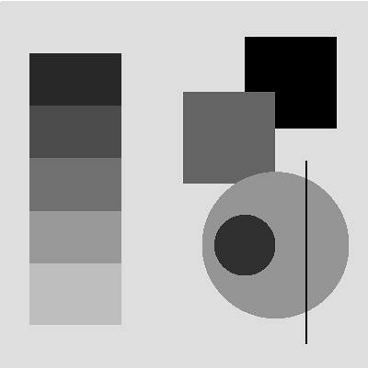
\includegraphics[width=\textwidth]{images/synthetic.png}
        \caption{Synthetic image, black on white.}
        \label{fig:syn1}
    \end{subfigure}
    ~ %add desired spacing between images, e. g. ~, \quad, \qquad, \hfill etc. 
      %(or a blank line to force the subfigure onto a new line)
    \begin{subfigure}[b]{0.45\textwidth}
        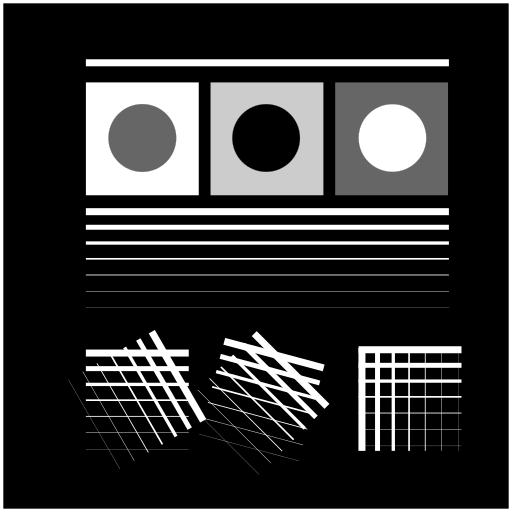
\includegraphics[width=\textwidth]{images/synthetic_2.png}
        \caption{Synthetic image, white on black.}
        \label{fig:syn2}
    \end{subfigure}
    ~ %add desired spacing between images, e. g. ~, \quad, \qquad, \hfill etc. 
    %(or a blank line to force the subfigure onto a new line)    
    \caption{Synthetic test images for edge detection algorithms. \subref{fig:syn1} shows various gray levels that require an adaptive algorithm. \subref{fig:syn2}
    shows more challenging edge detection tests that have crossing lines. Fusing these into full segments typically requires algorithms like the Hough transform.
    This is an example of using subfigures, with \texttt{subref}s in the caption.
    }\label{fig:synthetic}
\end{figure}

\clearpage

\subsection{Equations}

Equations should be typeset correctly and precisely. Make sure you get parenthesis sizing correct, and punctuate equations correctly 
(the comma is important and goes \textit{inside} the equation block). Explain any symbols used clearly if not defined earlier. 

For example, we might define:
\begin{equation}
    \hat{f}(\xi) = \frac{1}{2}\left[ \int_{-\infty}^{\infty} f(x) e^{2\pi i x \xi} \right],
\end{equation}    
where $\hat{f}(\xi)$ is the Fourier transform of the time domain signal $f(x)$.

\subsection{Algorithms}
Algorithms can be set using \texttt{algorithm2e}, as in Algorithm \ref{alg:metropolis}.

% NOTE: line ends are denoted by \; in algorithm2e
\begin{algorithm}
    \DontPrintSemicolon
    \KwData{$f_X(x)$, a probability density function returing the density at $x$.\; $\sigma$ a standard deviation specifying the spread of the proposal distribution.\;
    $x_0$, an initial starting condition.}
    \KwResult{$s=[x_1, x_2, \dots, x_n]$, $n$ samples approximately drawn from a distribution with PDF $f_X(x)$.}
    \Begin{
        $s \longleftarrow []$\;
        $p \longleftarrow f_X(x)$\;
        $i \longleftarrow 0$\;
        \While{$i < n$}
        {
            $x^\prime \longleftarrow \mathcal{N}(x, \sigma^2)$\;
            $p^\prime \longleftarrow f_X(x^\prime)$\;
            $a \longleftarrow \frac{p^\prime}{p}$\;
            $r \longleftarrow U(0,1)$\;
            \If{$r<a$}
            {
                $x \longleftarrow x^\prime$\;
                $p \longleftarrow f_X(x)$\;
                $i \longleftarrow i+1$\;
                append $x$ to $s$\;
            }
        }
    }
    
\caption{The Metropolis-Hastings MCMC algorithm for drawing samples from arbitrary probability distributions, 
specialised for normal proposal distributions $q(x^\prime|x) = \mathcal{N}(x, \sigma^2)$. The symmetry of the normal distribution means the acceptance rule takes the simplified form.}\label{alg:metropolis}
\end{algorithm}

\subsection{Tables}

If you need to include tables, like Table \ref{tab:operators}, use a tool like https://www.tablesgenerator.com/ to generate the table as it is
extremely tedious otherwise. 

\begin{table}[]
    \caption{The standard table of operators in Python, along with their functional equivalents from the \texttt{operator} package. Note that table
    captions go above the table, not below. Do not add additional rules/lines to tables. }\label{tab:operators}
    %\tt 
    \rowcolors{2}{}{gray!3}
    \begin{tabular}{@{}lll@{}}
    %\toprule
    \textbf{Operation}    & \textbf{Syntax}                & \textbf{Function}                            \\ %\midrule % optional rule for header
    Addition              & \texttt{a + b}                          & \texttt{add(a, b)}                                    \\
    Concatenation         & \texttt{seq1 + seq2}                    & \texttt{concat(seq1, seq2)}                           \\
    Containment Test      & \texttt{obj in seq}                     & \texttt{contains(seq, obj)}                           \\
    Division              & \texttt{a / b}                          & \texttt{div(a, b) }  \\
    Division              & \texttt{a / b}                          & \texttt{truediv(a, b) } \\
    Division              & \texttt{a // b}                         & \texttt{floordiv(a, b)}                               \\
    Bitwise And           & \texttt{a \& b}                         & \texttt{and\_(a, b)}                                  \\
    Bitwise Exclusive Or  & \texttt{a \textasciicircum b}           & \texttt{xor(a, b)}                                    \\
    Bitwise Inversion     & \texttt{$\sim$a}                        & \texttt{invert(a)}                                    \\
    Bitwise Or            & \texttt{a | b}                          & \texttt{or\_(a, b)}                                   \\
    Exponentiation        & \texttt{a ** b}                         & \texttt{pow(a, b)}                                    \\
    Identity              & \texttt{a is b}                         & \texttt{is\_(a, b)}                                   \\
    Identity              & \texttt{a is not b}                     & \texttt{is\_not(a, b)}                                \\
    Indexed Assignment    & \texttt{obj{[}k{]} = v}                 & \texttt{setitem(obj, k, v)}                           \\
    Indexed Deletion      & \texttt{del obj{[}k{]}}                 & \texttt{delitem(obj, k)}                              \\
    Indexing              & \texttt{obj{[}k{]}}                     & \texttt{getitem(obj, k)}                              \\
    Left Shift            & \texttt{a \textless{}\textless b}       & \texttt{lshift(a, b)}                                 \\
    Modulo                & \texttt{a \% b}                         & \texttt{mod(a, b)}                                    \\
    Multiplication        & \texttt{a * b}                          & \texttt{mul(a, b)}                                    \\
    Negation (Arithmetic) & \texttt{- a}                            & \texttt{neg(a)}                                       \\
    Negation (Logical)    & \texttt{not a}                          & \texttt{not\_(a)}                                     \\
    Positive              & \texttt{+ a}                            & \texttt{pos(a)}                                       \\
    Right Shift           & \texttt{a \textgreater{}\textgreater b} & \texttt{rshift(a, b)}                                 \\
    Sequence Repetition   & \texttt{seq * i}                        & \texttt{repeat(seq, i)}                               \\
    Slice Assignment      & \texttt{seq{[}i:j{]} = values}          & \texttt{setitem(seq, slice(i, j), values)}            \\
    Slice Deletion        & \texttt{del seq{[}i:j{]}}               & \texttt{delitem(seq, slice(i, j))}                    \\
    Slicing               & \texttt{seq{[}i:j{]}}                   & \texttt{getitem(seq, slice(i, j))}                    \\
    String Formatting     & \texttt{s \% obj}                       & \texttt{mod(s, obj)}                                  \\
    Subtraction           & \texttt{a - b}                          & \texttt{sub(a, b)}                                    \\
    Truth Test            & \texttt{obj}                            & \texttt{truth(obj)}                                   \\
    Ordering              & \texttt{a \textless b}                  & \texttt{lt(a, b)}                                     \\
    Ordering              & \texttt{a \textless{}= b}               & \texttt{le(a, b)}                                     \\
    % \bottomrule
    \end{tabular}
    \end{table}
\subsection{Code}

Avoid putting large blocks of code in the report (more than a page in one block, for example). Use syntax highlighting if possible, as in Listing \ref{lst:callahan}.

\begin{lstlisting}[language=python, float, caption={The algorithm for packing the $3\times 3$ outer-totalistic binary CA successor rule into a 
    $16\times 16\times 16\times 16$ 4 bit lookup table, running an equivalent, notionally 16-state $2\times 2$ CA.}, label=lst:callahan]
    def create_callahan_table(rule="b3s23"):
        """Generate the lookup table for the cells."""        
        s_table = np.zeros((16, 16, 16, 16), dtype=np.uint8)
        birth, survive = parse_rule(rule)

        # generate all 16 bit strings
        for iv in range(65536):
            bv = [(iv >> z) & 1 for z in range(16)]
            a, b, c, d, e, f, g, h, i, j, k, l, m, n, o, p = bv

            # compute next state of the inner 2x2
            nw = apply_rule(f, a, b, c, e, g, i, j, k)
            ne = apply_rule(g, b, c, d, f, h, j, k, l)
            sw = apply_rule(j, e, f, g, i, k, m, n, o)
            se = apply_rule(k, f, g, h, j, l, n, o, p)

            # compute the index of this 4x4
            nw_code = a | (b << 1) | (e << 2) | (f << 3)
            ne_code = c | (d << 1) | (g << 2) | (h << 3)
            sw_code = i | (j << 1) | (m << 2) | (n << 3)
            se_code = k | (l << 1) | (o << 2) | (p << 3)

            # compute the state for the 2x2
            next_code = nw | (ne << 1) | (sw << 2) | (se << 3)

            # get the 4x4 index, and write into the table
            s_table[nw_code, ne_code, sw_code, se_code] = next_code

        return s_table

\end{lstlisting}

%==================================================================================================================================
\chapter{Evaluation} \label{evaluation}

In this chapter, we outline the procedure used in evaluating the mobile application, 'GradReflect', 
with the aim of answering the research questions proposed in Chapter 1, whilst also identifying some 
potential areas for improvement. Some of these were implemented and can be seen in the program
as described in section \ref{implementation}. Others are listed in the future work in section (ADD FUTURE WORK SECTION REF)
either due to time contraints, or because they were seen to be outwith the scope of the project.
\par 
We present the results of the 
usability experiment and the following surveys that were conducted and discuss how these 
answer the questions and relate to the wider literature of graduate attributes. 

\section{Aims} \label{evalAims}

While our overall aim was to create a mobile application to capture reflections on when and where
students have exercised their graduate attributes, chapter 1 also outlined the extended aims of creating
an app that will assist users in making deeper reflections and developing their skills further using 
Cognitive Behaviour Therapy techniques (CBT). This is, however, a broad aim that would require a long-term 
experiment that is outwith the scope of this project to definitely answer it. Instead, this aim has been 
broken down into a series of smaller research areas that will contribute towards answering the larger topic:

\begin{itemize}
    \item We wish to establish that this application is easily usable and satisfying 
    for students to make reflections and navigate through to make either written or 
    audio formatted reflections. 
    \item As an extension to the previous aim, we wish to understand if users could see themselves using this 
    application again in the long-term. This will give insight into the long-term applications of this project, 
    continued use of this application could result in continued development of these skills and increase the employability
    of the students.
    \item Lastly, we also wish to establish whether students found it helpful and easy to reflect on their
    experiences. Does an application like this aid their self-analysis? Does each section of the app 
    contribute to this understanding and reflection?
\end{itemize}

\section{Personal Evaluation}
Before conducting any evaluations with participants selected from a sample of potential users, a stage of self-evaluation
was carried out. This was done to identify any usability problems before any participants were asked to evaluate and use 
the application. 
\par 
To gain an insight into how the users would interact with the application, we installed the application onto our own device
and went through each section of the application as a user would, make several of recordings, either audio or written, 
examining the statistics and making use of the different areas of information on how to reflect and what these skills are.
\par 
Following this we conducted an informal heuristic evaluation using Jakob Nielsen’s “Ten Usability Heuristics” (REFERENCE). 

\subsection{Results}
From analysis made in relation to the usability heuristics we were able to identify changes that should 
be made to the app before allowing participants to have access for their evaluations. 
These changes were as follows:
\begin{itemize}
    \item Addition of a 'Cancel Note' button when creating a note
    \item Addition of an 'Edit' button on the notes list view, this was intended to make the application more intuitive
    for non-apple users who could potentially not be familar with the typical 'swiping' gesture.
    \item Changed the position of the 'Edit' button to remain consistent with the position in the notes list view
\end{itemize}

\section{Monitored User Evaluation}

The monitored user test had the aim of allowing users to give feedback on easy it was to use to the interface. 
After signing consent forms, participants then had the opputunity to interact with the application on the simulated iPhone, 
prebuilt into the XCode IDE, through a video conference where they were given remote control. This was chosen as it 
would give the users the chance to get, as close as possible, hands-on experience of the application. This would be 
more beneficial than the typical study, where users would only be able to review video demonstrations of the app, as 
it would give more insight into how a user will interact with the application in a real-world environment. This 
is something that without giving the application to actual users would be largely unpredictable. 
\par 
Conducting this study over video conference also meant the evaluations were able to be recorded, allowing for review 
of the experiment to gain further insight into the reactions and comments the participants made. 
Additionally, this would allow participants with a device or background of any mobile operating system to 
be included within the survey. This allowed for insight into whether this application would be intuitive for all 
users, implying that the same or similar designs could be taken to create an application over other platforms. This
would benefit any future studies into the use of a mobile application employing CBT techniques to capture graduate attributes 
reflections. 
\par 
The monitored aspect of this evaluation will allow for a better understanding of how the users interacted
with the application, and not just their final results and opinion. Observing the participants will allow the us to 
witness any hesitations, difficulties or mistakes that are made during the use of the app that they would 
perhaps forget when it came to them answering the usability survey. A monitored evaluation also provided the oppurtunity
for the participants to ask any questions if they were stuck on any of the tasks, and 
to use a 'Think Aloud' approach as they were encouraged to voice any of their thought processes
or difficulties as they used they app, should they wish to. This allowed any points of interest to noted by the 
experimenter alongside the participants actions. (ADD IN SCHOLAR REFERENCE DISCUSSING THE BENEFITS OF THINK ALOUD)
\par 
Upon entering the video conference, participants were again asked if they were comfortable with being recorded for the evaluation. 
Once they agreed, the evaluation began recorded and the participant was read an introductory script which gave insight into how
the evaluation was going to be carried out, again, providing them the oppurtunity to withdraw at any point in the evaluation.
\par 
Participants were then given some time to familiarise themselves with the application and the controls of using this application
via their mouse and computer. This was key as using a mobile application is a foreign concept to most people. Allowing for 
this time would prevent the participant evaluating on the simulator, rather than on the application itself. 
\par 
Following this users were then asked to complete a set list of tasks. These tasks were created to make sure that the participants 
explored through every section of the application and therefore having a better view of the application as a whole, giving the oppurtunity
to voice any opinions on features they liked or disliked, or what they were struggling with. Participants were given any additional help 
if needed during this evaluation if they had difficulties using the simulated phone.
\par 
At the end of the monitored evaluation users were debriefed and given the opputunity to make any comments about their experience
of the application.
\par 
\par 
For this evaluation a total of 8 participants were gathered from a convenience sample of students from various degrees, 
consisting of both young and mature students. 
\par 
The majority of participants were in the age range of of 18-24, with this range having 5 participants. There were 
3 participants in the 25-34 range.
\par 
A total of 4 participants identified as female, and 4 participants identified as male.
\par 
Most students had a strong technical background. A total of 4 participants are currently studying a university level 
qualification in computing. The remaining 4 participants has never studied a qualification in computing.
\par 
Having participants from degrees other than Computing Science allowed for generalisation of the results to give insight
over how any student will react and interact with this application. Having a sample made only out of Computing Science
students may give the results an unfair bias as these students are more likely to be quick to understand 
various layouts of interfaces and would be quick to navigate through and understand most applications. Using students from 
multiple degrees and mature students also, meant that we could give insight into how this application could be useful to
any student of any background or experience, as the target demographic for this application is students who will need to develop these
skills for the workplace.

\subsection{Task explanation}

The tasks that users were given involved exploring the features on each view of the application.

\textbf{Home Page} Users started here as this allowed them to familiarise themselves with the skills that they would need
to be able to reflect on in the future. 
\par 
\textbf{Settings Page} Users were asked to progress to settings as this would allow them to view the background features that would 
be useful for a first time user. These tasks involved asking the user to explore the Useful Links, About GradReflect, toggling the
notifications and dark/light theme of the application. This allowed users to view and familiarise themselves with some additional 
information that could help them in future use of the application and show where they would need to go to customise the app, as well
as reading about the general purpose of the application.
\par 
\textbf{Notes Page} Users were then asked to create a note based on the skill teamwork, and given the option of using any additional
aids should they need to. This tested the users ability to be able to reflect easily with the aids and prompts given to them on the 
note taking sheet and whether this was simple for them to carry out. Users here were also asked to review this note and to attempt to
create a note with no name. This was to allow users to familiarise themselves with the how they would be able to look back on previous
notes and experience error prevention within the application. Finally, in this section users were asked to use the search functionality
to allow the user to customise their list view.
\par 
\textbf{Statistics Page} In this section of the application users were asked to view the statistics based on the note they had
just created. This was to allow users to experience this feature of the application and to allow for evaluation on the usefulness
of this later in the survey. Following this, users were asked to delete the note they had created, testing how intuitive it is
for a user to be able to remove a note they had made.
\par 
\textbf{Recordings Page} Once users had navigated to this section, users were asked to create a note with and without a name.
This was to show users the different naming options they could follow and allow for evaluation on this by them. The participant
then had to playback and delete a recording, again testing to see how easily users would be able to do this.

\subsection{Monitoring}
Participants were observed throughout these tasks. The recordings of the evaluations were then reviewed and notes were taken
on any difficulties the users encountered or any issues or positive comments they had discussed with the observer about the
application. 
\par 
Following the completion of the tasks, participants were asked for any comments they wanted to make about their 
experience with the application. These were also taken note of and kept for analysis.

\subsection{Results}

The recorded monitored evaluations with our participants were reviewed and any notable difficulties or 
comments from the participant were transcribed. To group together and identify major themes each notable 
response was categorised under the task where it occured. For certain tasks, users encountered no difficulties 
and made no comments. We present the most significant themes that were found during the evaluation. When 
referring to specific participant responses, we will refer to them by their ID number to maintain their 
anonymity.
\par 


\textbf{Initial exploration of app}
\par 
When participants were given the oppurtunity to explore the application it was noted that every participant
scrolled through some, if not all, of the skill cards. With some participants navigating through every 
view and component of the application before beginning the tasks. Participant 1 noted that they thought
having a section for audio recordings was "cool". Participant 2 voiced that they enjoyed the images that
accompanied the skill cards, echoed by participant 8 during their evaluation. Participant 2 also stated 
that they liked that the statistics page also included the statistic of average word count over all notes created.
Participant 8 also stated that they thought the app was overall very "cool".
\par 

\textbf{Reviewing the descriptions of the skills}
\par
Participants overall appeared to enjoy the descriptions of the skills. Several of the participants noted that 
they enjoyed the short descriptions of the skills, for example, participant 1 stated that there was "good use 
of examples", the descriptions were not "long-winded", and that the images were useful and enjoyable, participant 4 
also stated that they enjoyed the images. Participant 2 stated that
the images helped them to further understand the descriptions of the skill. Participant 6 also stated that they liked
the "simplicity" of the app descriptions, and stated "there's enough information without overwhelming you by 
having to read a big essay to be able to understand".
\par

\textbf{Following the useful links}
\par
In this task, participants were to follow links from the app to useful pages about graduate attributes, the project
GitHub and Glasgow University's Moodle page. This required the participants having to be able to close the app Safari
on the mobile and open the GradReflect application again to return. Participants 2, 4, and 5 here struggled to be able
to do this due to the need to click an alternative 'Home' button that was responsible for closing any app. However, this
is due to the nature of conducting the experiment over a video conference and is a reflection on the simulator and 
not the application. Participant 2 also noted that they liked the link to the university Moodle page.

\textbf{Reading the 'About GradReflect' page}
\par
Whilst reading the 'About GradReflect' page participant 6 stated that they liked "the part that said 
'notes require a title', as it helps if you cant understand why something isnt working and theres an answer available" and
further stated that there was "a lot of good information" on this section of the app. Participant 7 noted that due to the 
application being on a laptop it "felt weird to have the text all the way up to the sides, but if it was actually on
a phone i would like it up to the sides"

\textbf{Turning on and waiting for the notification}
In this task, users only had to wait 10 seconds due to notification being a proof of concept for testing and evaluative
purposes. However, again due to this task requiring users to close the application, some participants struggled with 
locating the simulator button to close an app, this included participant 3 and 8. Participant 2 noted that the ability to
have notifications was "cool"

\textbf{Changing the theme of the app}
\par 
Overall, participants seemed to enjoy this feature and it's customisability. Participant 2 and 8 specifically stated that 
they enjoyed having this feature.

\textbf{Creating and saving a note}
\par 
In this task, participants frequently made use of the question helper buttons, with 7 out of 8 participants using them
at least once. Participant 3 needed clarification of where to enter their notes. Participant 4 initially attempted
to create a note by clicking the 'Edit' button on the notes list view, but quickly realised where the 'Add note' button
was located and went to use that instead. Participant 5 struggled with scrolling on the page due to having to hold
down with their cursor, this was due to it being a virtual phone evaluation. Participant 6 when using the emotion
slider initially attempted to click on the scale where they wanted to adjust the slider too, however, when this did not 
work they knwo they instead had to drag the scale to their desired position. Participant 7 struggled to see where
to select the skill type but after asking they were able to choose the skill.

\textbf{Reviewing a note}
\par
Participants did not struggle to open the note after creation, however, participant 1 stated that they wished they were able
to scroll with their mouse instead of holding down their cursor to push the screen up. This is due to conducting the 
evaluation virtually as the simulated phone requires the mouse to act as a finger would on the screen. Participant 6 noted 
she had not answered the questions they way she had intended as she had not read the questions properly, and that if she
was to do another note she would know better how to asnwer them.

\textbf{Reviewing the statistics}
\par 
During the review of their notes, participant 2 stated that they enjoyed the statistics as they are helpful when evaluating 
yourself and whether you are good and bad at something, especially with the emotion and how much you have written, getting 
an idea of how much you have written and how much detail help to get an idea of your own thoughts and what to do moving forward.

\textbf{Deleting a note}
\par 
In this task, some users struggled with understanding how to delete a note, when asked to do this participants 1, 3, 5, 6, and 
8 attempted to delete the notes by opening the reviewing view of a note and scrolling to the bottom, however after realising
there was no button to delete a note here they found the 'Edit' button and saw that this would let them delete notes. 

\textbf{Creating a named recording}
\par 
During this section participant 1 at first attempted to record a note by holding down on the record button instead of just tapping 
it, however, after seeing this did not create a note and just started the recording after releasing the button, the participant tried 
again but the note did not save. Once they then renamed and created a recording they were able to create a note. No other issues
were encountered from participants with creating a recording.

\textbf{Playback a recording}
\par 
During this task further issues were encountered due to the necessity of conducting this evaluation over a video conference. 
When creating a recording the simulated phone was connected to the experimenter microphone and therefore only faintly 
picked up what the participants were saying. The participants were then not able to hear back any audio from the simulator
as th video conference was not sharing any audio from the experimenters computer device, however, the experimenter was
able to hear back the recordings quietly, ensuring that the participant knew that their recording had worked. No participants
had any issues carrying out this task.

\textbf{Comments given by participants at the end of the tasks}
\par 
At the end of the tasks participants were given the oppurtunity to voice any comments about their experience. Participant 2
stated they found it easy to use, especially as it used familiar iOS practices. Participant 4 noted that the app was easy to 
use and was intuitive and laid out well, as well as being user friendly. They also stated they would use it as a space to reflect 
about what work they are doing to think over things at the end of the day. Participant 5 said the app was seamless, worked really 
well, and was straightforward for the user. Participant 6 stated it was a very good app as it was nice and easy to use, 
and they could navigate easily and there were clear labels. They went on to say they liked the helper buttons as they helped 
give something to work with in terms of answering the question. Participant 7 said that when deleting any notes or recordings they
thought iOS users would swipe rather than click 'edit', however, this was an option that was also available. Participant 8 stated
that they liked it, thought it was easy to navigate, they also stated the first time using an app is diffcult, especially 
virtually, but if they had the app they would continue using it as it did seem really simple.

\subsection{Overview}

The monitored evaluation highlighted several areas where the application had met the aims of the project.
\par 
\textbf{Creating an application to capture reflections on graduate attributes:} Every participant was able to make a note
about their experiences and reflections on a time they used the skill teamwork
\par 
\textbf{Allow users to create a note via written or audio form:} All users were able to make a note with both written and audio
formats. This shows that for future use of this application users would be able to make a choice over which method is the 
most convenient for them to reflect. Having this ability to make reflecting easier could enocourage more users to reflect.
\par 
\textbf{Capability for reminders:} All users were able to turn on the notifications that sent out a reminder to the participant
10 seconds after clicking, with some participants specifically stated they enjoyed this feature.
 In future work for this application and in a real-world setting users would be able to choose when this 
notification was sent. However, for this evaluation it was more useful that the participants were able to immediately see the 
notification so they could return to the application and continue with the evaluation.
\par 
\textbf{Create a usable application:} From the results of the monitored evaluation, it can be seen that the majority of users faced no issues when using the application,
and overall enjoyed their experience. Participants noted several areas that they particularly enjoyed, these comments highlighted 
areas where the application met the usability standards before the surveys, containing questions directly relating to these standards,
was completed. The minimalist design of 
the skill cards made clear to the users what was important when reflecting using the application, with the accompanying images
helping to deepen understanding. In the settings view users enjoyed the customisability the application provided through the ability to
change the theme, also noting that the application provided good documentation within it to help with any issues users would encounter.
\par 
Within the concluding statements of the evaluation, several participants stated the application as being intuitive, user-friendly.
During the survey, some participants made statements about how they would use the app in the future, for example, when they would
use the statistics page, how they would get more familiar to the app the more they used it, and how in the future they felt they 
would answer the questions with better responses. This demonstrates that the participants were showing an interest in how this app
could be useful to them in the future
\par 
\textbf{Aid reflection:} During this evaluation, the applications ability to assist in reflection was highlighted as the users 
created their first note. The question helper buttons were used by the majority of participants, they were seen to ground the user
in what they were meant to reflect on and after users had read these they appeared to be able to quickly make a reflection based on this.
The prompts followed the CBT approach, which from section (ADD THE EXPERIMENT SECTION NAME) has shown to encourage deeper reflections.
Users were also assisted through the descriptions given from the skill cards, participants stated that these descriptions gave them a
better understanding of what these skills are, and therefore they should be able to make better reflections on these skills as they become
more aware of what they are and when they are using them.
\par 
\textbf{Future work identified by observing participants}
\begin{itemize}
    \item Allow users to delete a note from within a note review view.
    \item The emotion slider could allow users to click where they want the slider to go, as well as being able to drag.
    \item Make the button to delete notes clearer to the users, make it red with a 'delete notes' label next to it, include 
    in the app description that users are able to both click the edit button, and swipe in the typical gesture iOS apps are able to do.
    \item 
\end{itemize}
All of these hanges make sense to be added to the application, and can be seen as future work.


\subsection{Limitations}

While the design of out evaluation allowed us to answer the reasearch questions we had previously defined, there are a number
of ways in which the study could be improved.
\par 
Although we are studying how students would use this app on their own mobile devices, the decision
was taken to run these experiments in a controlled setting over a Zoom conference. This was due to this being an iOS application,
meaning it would require an apple developer license to 
be able to widely disperse this application through the apple app store. This meant that to test
this application on their own device, users would need to be able to connect their phone to the experimenter's Apple computer, 
so that the application could be installed. However, this project was conducted
during the COVID-19 pandemic, meaning it would not be safe to meet with experiment participants
for testing purposes and to install locally on their device, as this would put them at risk of exposure to the virus. 
\par 
Conducting this experiment virtually allowed us to test the application during the COVID-19
pandemic, however, this may have affected the behaviour exhibited by participants. 
For example, users were not able to use the controls of the 
phone as easily and at times struggled, instead having to opt for a 'Home' button outside of the simulator to be able to close the application instead
of the typical 'swiping' from the base of the phone to close an app. This at times created frustration for the participants as 
they attempted to use to option that they would on a physical phone. This environment also caused issues when a participant was
not able to access the additional 'Home' button of the simulator as Zoom had a 'Remote control' taskbar display on top of this 
button, causing confusion and delay as the participant realised they needed to remove this taskbar on their device to view the
'Home' button. Therefore, further studies should be conducted that allow a participant to be able to install on their device 
or use an experimental physical device to evaluate the application. This would ensure that the behaviour observed is representative 
of the behaviour that would be exhibited should the app be usable in-person.
\par 
Additionally, the participants came from a convenience sample of friends and family members. Therefore this could have also impacted
the behaviours exhibited by the participants. Further studies should take care to conduct their experiment using a more representative 
population of unknown participants, to ensure the results can be generalised.


\section{Post-study Survey}
Following the completion of the monitored evaluation, participants were then asked to fill in a post-study survey. This
survey had two sections.
\par 
In the first section of the survey we followed Nielsen’s approach of conducting a heuristic evaluation
utilising his approach of identifying and evaluating ten usability areas (REFERENCE from hci project).
Participants would response to these questions via a series of statements based on whether they agree or disagree on the 
usability. These ranged from "Strongly disagree' to 'Strongly agree'. These were intended to give deeper insight
into how users felt about thier experience with the app, these would give better insight than the personal evaluations
that were conducted also using Neilsons heuristics, and identify if there were any issues that had not been picked up or areas
that could be further improved on. 
\par 
In the second section of this survey we asked questions that related more towards the features of the application. We wanted
to establish their general feeling towards the application by asking how they found using different features of the app,
if they found it quick to make a note, if they would be likely to use the app again, and if there were enough aids to help
them reflect. The specfic features we asked about were the audio recordings and the statistics sections. These were sections
that were added to the requirements of the application to extend it's use cases, and therefore insight into participant's reaction 
to these features would demonstrate whether they were necessary or would go unused. 

\subsection{Task explanation}

Participants were asked to fill in a survey based on these usability standard mentioned in section (ADD REF), these questions
can be seen in the appendix at section (ADD REF)

\subsection{Results}
 
The average response to each of the usability heuristics was gathered and put into individual graphs, that can be seen in the appendix
(STATE THE SECTION IN THE APPENDIX), and then processed further by taking the average response to each usability heuristic.
\par 
This graph can be seen in figure (REFERENCE)
\par 
Most participants strongly agreed that the system was usable and satisfying. For 8 out of the 10 usability
heuristics, participants all strongly agreed that the app entirely met these standards. 
However, 3 of these heuristics, consistency and standards, recognitions rather than recall and error prevention, did not score as highly.
\par 
From this first section of the survey, participants were also able to explain their motivation behind their scorings. 
These open-ended questions were analysed and major themes were identified.
\par 
\textbf{Ease of Use} When giving comments on their answers many participants stated explicitly how they thought the application was 
easy to use, intuitive and clearly laid out, with one participant even stating "Simple to understand for a technophobe like me". 
Other users mentioned that the navigation was clear to follow, with buttons being placed logically so they were easy to find,
and the application used features that were very familiar to typical iOS design and other similar applications. Error messages 
were also stated to be easily identifiable and understandable, users stated that they were 
made clear what the issues were and how they should be solved. Participants also noted that they appreciated the extra help icons 
as they gave more direction to the users on how they should be answering the questions.
This shows that generally users did not find using the application difficult, making for an enjoyable experience.
\par 

\textbf{Issues users had with the application and scorings} For the areas where users did not strongly agree with the heuristic they were
able to give explanations for their answer in the comments. The heuristics for consistency was given 2 agree scores. One
participant stated "I am an adroid user" as their explanation. This could be due to the app mostly following native to iOS design
practices and not being familiar for someone who has experience in only android phones, this could make it more difficult for a user.
The other participant stated as their comment for why they scored consistency as agree "The app used a consistent colour scheme 
throughout and consistent and intuitive navigation options between and within the apps pages and sections. The settings page was 
also made to look similar to the operating systems main settings page. this consistency with other systems made it easy to understand 
its purpose." This does not give a clear indication of why this participant did not score this heuristic as highly as the other 
participants.
\par 
Recognition rather than recall also did not score as highly, with one user scoring this as agree and stating "This was easy to 
understand throughout. On the create note page I scrolled down to understand the full extent of the form and what was required 
of creating a note before completing it." This shows that for this user they were unsure of what would be necessary for them to
reflect before they had looked at the note creation view, meaning that on first viewing of this page the user could potentially 
not be using this note creation to it's full potential. 
\par 
Another participant scored error prevention as neutral, however, this was not stated to be a negative review of the application
as the participant explained "I encountered no errors". This scoring could show that the user did not feel the need to rate this
attribute postively or negatively as they had not witness any errors within the application. 
\par 
\textbf{Future work identified by participants}
\begin{itemize}
    \item In the future, this application could be made cross-platform meaning it would be required to use less iOS design so that 
    it would be suitable for a user with experience with any operating system. Additionally, an android version of this application
    could be made seperately to also fit the needs of more users. 
    \item In the future, more descriptions of the questions users will have to answer and the depth of reflection needed from them 
    could be made more clear in the description of the application. Allowing users to preview what is expected of them before they 
    begin to reflect could help them be more prepared and leas to better reflections.
\end{itemize}
\par 
Following this section of the survey, users then had to answer question relating to their preferences and experience with the application
in general. 
\par 
The survey asked about specific features of the application and recurring themes were identified in each of the comments
for these questions. These questions were useful in targetting the aims of the project to find insight into whether the participants 
felt these were met.
\par 
\textbf{Creating an application to capture reflections on graduate attributes:} The first question asked the users how easy they found reflection. 7 out of 8 participants voted the application as very easy 
to reflect with, with 1 participant voting easy. This shows that for the majority of people, this application was overall 
very useful for users to reflect and provided enough assistance and prompts for the users to reflect on their graduate attributes 
without any issues. However, there is still room for improvement to make this process more seamless for every user.
\par 
\textbf{Allow users to create a note via written or audio form:} All participants stated that they felt the ability to create audio 
recording was useful, with several participants stating that they would be useful for quick and convenient reflections as they are 
less formal. One user stated that "The recording section, in particular, took very 
little time and effort to add to and often saying how you are feeling can make it more memorable, enhancing its usefulness.", showing 
the addition of this audio recording feature assists users in being able to reflect via more than one format, and that there is value
in being able to think out loud about graduate attributes. This ease of reflection could encourage users in the future to carry out 
more casual and frequent reflection. 
\par 
\textbf{Create a usable application:} When asked if users were able to quickly create a note, all participants voted yes. Users stated that
it was intutively designed and easy to just fill in the boxes. One user stated that the questions and prompts helped to break down
their thoughts easily. This shows that the design of the application and the use of the CBT line of questioning and prompts helps
the user to quickly be able make notes based on meaningful reflections. 
\par 
When asked if users would continue to use this application, all participants voted yes. In the comments for this question many participants
noted the ways they felt an application like this would be useful for them in the future. Two participants noted that this application
could be useful for future employment by helping you list the skills you have used that would be crucial to the workplace and help to 
develop their CV, with another participant also stating that it would help them to "see the skills I have developed outside of the 
basics of my degree focus". This shows that participants have identified the key uses for this application and how reflecting on and 
developing these skills is crucial to assist them in their future workplace. Another participant also noted other ways that this app could 
be useful stating "Reflection on what you are able to do and how you feel can be helpful for mental health and also inspire you in 
what you are currently doing", suggesting the application could be used in the future for further benefits than just to employability.
\par 
The majority of users also felt that the statistics page was also useful, with 1 participants stating "Stats aren't my strong point". 
Participants found this would assist in helping them focus on what skills the need to focus on and develop further, with one 
participant noting that it could be encouraging to see what skills have already been developed. This further extends the use cases of the 
application, allowing them to reflect more efficiently as they would be able to see the areas that are weaker. 
\par 
\textbf{Aid reflection:} When asked if participant felt there was enough assistance to aid reflection, all 8 participants voted 
yes. Participants specifically stated that the helper buttons were very useful and they appreciated the additional information to
prompt their reflections, as well as showing how they application was meant to be used. One participant specifically stated 
"I found the prompts helped me to think in a deeper way about the situation I was describing, it gave me time to think about 
my emotions/reactions." This shows that the application meets the needs of users to help them reflect in a more meaningful way.
This reflection would be useful in the future for users to develop their graduate skills further.
\par 

\textbf{Future work identified by participants}
\begin{itemize}
    \item Filtering the notes by clicking on one of the skill categories on the skill cards.
    \item Ability to set goals for number of reflections on a skill and receiving milestone achievements when these are met.
\end{itemize}

\subsection{Limitations}
One major limitation of this evaluation was that it could not have been conducted in person due to the COVID-19 pandemic. Future work
would be recommended to conduct interviews with particpants as this would allow for the interviewer to enquire further and follow-up
on the responses that the participants give. This would allows for further insight into what the participants think about their 
experience with the application.

\section{Overall}
\subsection{Verification of functional requirements}
\subsection{Verification of non-functional requirements}

\section{UI Tests}

In the future the application would require extensive UI and Unit testing to be released for general use by the public, however, due
to the aims of my project only one UI test was created to give a proof of concept idea for the tests that should be created for future
work. The UI feature that has been tested is the users ability to create and save a written note. This was chosen as this is the 
basic necessary requirement for the application to run functionally. 
\par 
If you visualise, follow the basic rules, as illustrated in Figure \ref{fig:boxplot}:
\par 
See the file \texttt{guide\_to\_visualising.pdf} for further information and guidance.
\begin{figure}
    \centering
    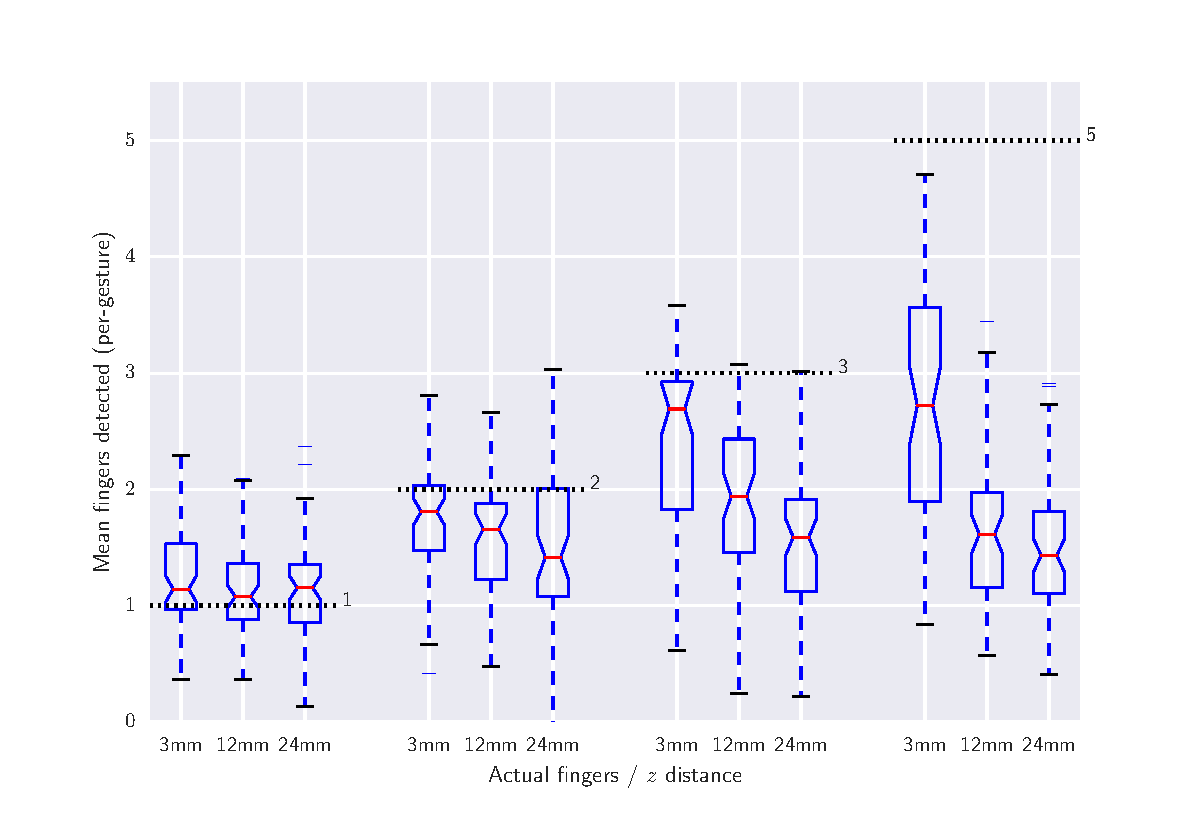
\includegraphics[width=1.0\linewidth]{images/boxplot_finger_distance.pdf}    

    \caption{Average number of fingers detected by the touch sensor at different heights above the surface, averaged over all gestures. Dashed lines indicate
    the true number of fingers present. The Box plots include bootstrapped uncertainty notches for the median. It is clear that the device is biased toward 
    undercounting fingers, particularly at higher $z$ distances.
    }

    % use the notation fig:name to cross reference a figure
    \label{fig:boxplot} 
\end{figure}


%==================================================================================================================================
\chapter{Conclusion}  

Summarise the whole project for a lazy reader who didn't read the rest (e.g. a prize-awarding committee).
Summarise briefly and fairly. Indicate what future work could be done, but remember: you won't get credit for things you haven't done.
What did i do during this project
basically go over the intro and the background and problem statement all over again
Future work
Go over how my project could be improved in the future
If i had more time on the project what i could further accomplish
Eg : could have further done tests to see whether over time users felt that they had improved on their skills, are they more aware of their skills etc
Eg : ways i could have made the app more useful, summarise the ways from the eval summaries that i could have made the app itself better
Could use a tab bar instead of the page navigation
Could use a floating '+' button instead to make a new note/recording
Personal reflections
Why did i choose swift
What did i learn by using swift that will help me in the future
Perhaps talk about how my confidence grew through using a language that was entirely new to me, gained technical skills and within myself developed the graduate attributes that i was studying
Talk about some of the difficulties i faced with it being a relatively new development method
The project was well suited to me as i enjoy HCI and the personal interaction people can have with technology and provide a better experience in their life, and about psychology aspects
Gained an interest in app development and will now further delve into this and perhaps in future create the same type of application for a webapp to see if that could provide access to a further range of people other than iOS users.  
Summarise the whole project for a lazy reader who didn't read the rest (e.g. a prize-awarding committee).


\section{Guidance}
\begin{itemize}
    \item
        Summarise briefly and fairly.
    \item
        You should be addressing the general problem you introduced in the
        Introduction.        
    \item
        Include summary of concrete results (``the new compiler ran 2x
        faster'')
    \item
        Indicate what future work could be done, but remember: \textbf{you
        won't get credit for things you haven't done}.
\end{itemize}

%==================================================================================================================================
%
% 
%==================================================================================================================================
%  APPENDICES  

\begin{appendices}

\chapter{Appendices}

Typical inclusions in the appendices are:

\begin{itemize}
\item
  Copies of ethics approvals (required if obtained)
\item
  Copies of questionnaires etc. used to gather data from subjects.
\item
  Extensive tables or figures that are too bulky to fit in the main body of
  the report, particularly ones that are repetitive and summarised in the body.

\item Outline of the source code (e.g. directory structure), or other architecture documentation like class diagrams.

\item User manuals, and any guides to starting/running the software.

\end{itemize}

\textbf{Don't include your source code in the appendices}. It will be
submitted separately.

\end{appendices}

%==================================================================================================================================
%   BIBLIOGRAPHY   

% The bibliography style is abbrvnat
% The bibliography always appears last, after the appendices.

\bibliographystyle{abbrvnat}

\bibliography{l4proj}

\end{document}
